\chapter{声学拓扑晶体绝缘体的理论建模方法}
\section{引言}

要在声学系统中构造类拓扑绝缘体并观察其拓扑效应,离不开基本的声学结构,如散射体,共鸣腔等。本质上,我们需要使用一些传统的声学结构,使得声波满足的控制方程和边界条件与凝聚态物理中的拓扑绝缘体理论有着高度的相似性。其设计思路完全可以是基于直觉的,我们可以基于理论模型的对称性来设计相仿的声学结构,然后依据直觉尝试调控结构参数来调节相互作用的大小。例如,当两个腔体之间的距离越近,连接导管横截面积越大,我们可以认为腔体间的相互作用越大,进而根据这一猜想调整结构直至出现预期的拓扑现象。这一过程可以通过有限元仿真来完成。
但是,仅仅借助经验的尝试和仿真工具,虽然能在声学系统中设计结构观测到一些拓扑效应,却还不足以揭示声学系统和凝聚态理论之间的深刻联系。一方面,声学拓扑绝缘体的设计离不开一些传统的声学结构,而传统的声学研究已经对其中一些结构已经有了一套比较系统的建模方法。另一方面,从研究尺度而言,在波长远大于结构尺寸的时候,分布参数的声场可以等效为集总参数系统,这时可以借助等效电路来研究离散的声学结构参数。这一思想与电子系统中的研究离散格点的物理量不谋而合。除此之外,当波长接近与某些结构尺寸的时候,这时亚波长的假设可能不适用。这种情况下,我们仍然可以通过单个规则结构的边界条件,计算其格林函数以获得其声场情况,然后进一步研究结构间的耦合,来获得近似模型。

本章的内容是介绍以上两种建模方法的研究思路,主要内容如下:在2.2节中,我们阐述了声电类比方法,其中包括腔管声学结构的等效电路元件及其适用条件和等效电路的连接方法;在2.3节中,我们介绍了腔体的简正模式和格林函数之间的联系,据此可以通过边界情况和格林函数积分求得声场分布;最后,2.4节是本章内容的小结。

\section{声电类比方法}

由于我们在用声学实现拓扑效应时,很多情况下是利用腔管共振结构实现声学结构和电子晶格结构的对应。而在声学研究中,电声类比是研究这类结构的一种常用方法。它适用于结构尺寸远小于波长的情况,是一种将集总参数的电路系统和声学系统进行类比分析的有效手段。它基于电学和声学在某些物理特性和数学描述上的相似性,建立起两者之间的对应关系,从而借助电学中成熟的理论和分析方法来研究声学问题。
在这种类比中,电学中的电压、电流、电阻、电容、电感等概念分别与声学中的声压、体积速度、声阻、声容、声感等概念相对应。通过电声类比,我们可以将复杂的声学系统转化为等效的电学电路模型,利用电路分析的方法来求解声学系统的特性,因此本节首先介绍这种方法。

\subsection{声容、声质量和声阻}

\begin{figure}[h!]
  \centering
  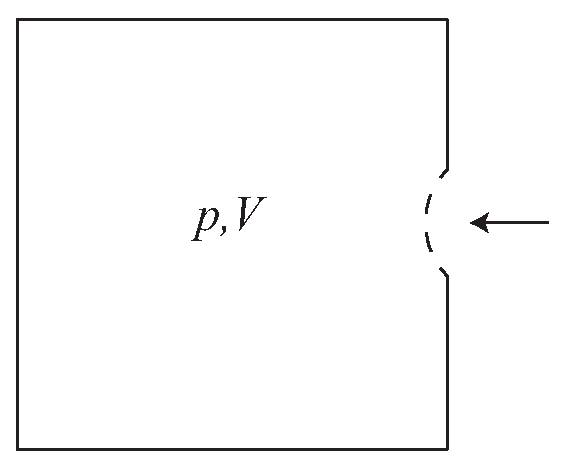
\includegraphics[width=0.5\textwidth]{images/fig2-1.eps} 
  \caption{声容示意图。 }
  \label{fig_2_1}
\end{figure}

首先,我们考虑腔体结构。对于一个壁面为刚性边界且带开口的腔体,当腔体里面的空气振动时,其声压和体积变化存在着某种函数关系。我们假设开口较小,并且且波长远大于结构尺寸时,这种关系往往可以被线性化的。我们可以把这样的结构称为声容,如图 \ref{fig_2_1}。声容的推导从绝热近似的状态方程出发,假设声波传播过程为绝热过程,则
\begin{equation} \label{eq2-1}
  pV^\gamma = \text{常数},
\end{equation}
其中 \(p\) 为气体压力,\(V\) 为气体体积,\(\gamma = C_p/{C_v}\) 为绝热指数。对该公式取对数后对时间求导,得到
\begin{equation} \label{eq2-2}
  V^\gamma \frac{dp}{dt} + \gamma p V^{\gamma-1} \frac{dV}{dt} = 0,
\end{equation}
整理为
\begin{equation} \label{eq2-3}
  \frac{dp}{p} + \gamma \frac{dV}{V} = 0,
\end{equation}
假设声波的压力和体积变化为微小量,即
\begin{equation} \label{eq2-4}
  p = p_0 + \Delta p, \quad V = V_0 + \Delta V,
\end{equation}
代入后忽略高阶小量项,得
\begin{equation} \label{eq2-5}
  \frac{\Delta p}{p_0} = -\gamma \frac{\Delta V}{V_0},
\end{equation}
从中可得体积变化和压力变化之间的关系为
\begin{equation} \label{eq2-6}
  \Delta V = -\frac{V_0}{\gamma p_0} \Delta p,
\end{equation}
声容 \(C_a\) 定义为单位压力变化引起的体积变化:
\begin{equation} \label{eq2-7}
  C_a = \frac{\Delta V}{\Delta p},
\end{equation}
将上述关系式代入后得到
\begin{equation} \label{eq2-8}
  C_a = \frac{V_0}{\gamma p_0},
\end{equation}
进一步结合声速的定义
\begin{equation} \label{eq2-9}
  c^2 = \frac{\gamma p_0}{\rho_0},
\end{equation}
将 \(\gamma p_0\) 替换为 \(\rho_0 c^2\),最终得声容的表达式
\begin{equation} \label{eq2-10}
  C_a = \frac{V}{\rho_0 c^2},
\end{equation}
这一公式揭示了声容取决于腔体体积 \(V\)、介质密度 \(\rho_0\) 和声速 \(c\),其中声容越大表示腔体对压力变化的响应越显著。

\begin{figure}[h!]
  \centering
  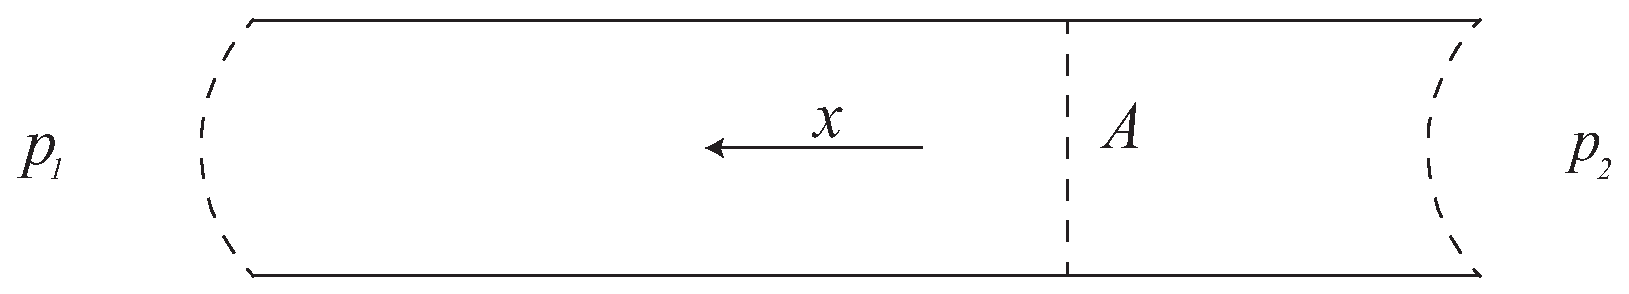
\includegraphics[width=1\textwidth]{images/fig2-2.eps} 
  \caption{声质量示意图。 }
  \label{fig_2_2}
\end{figure}

接下来,我们阐述短管里的空气声压和速度所满足的关系。当频率比较低,波长比较长的时候,短管的结构尺度远小于波长,我们可以认为短管里的空气是整体振动的,此时,我们可以把它视作质点,或者声质量,如图 \ref{fig_2_2}。声质量的推导从牛顿第二定律开始。假设在声学系统中,颈管内的空气柱被视为振动的质点,其运动遵循牛顿第二定律:
\begin{equation} \label{eq2-11}
  F = M \frac{d^2 x}{dt^2},
\end{equation}
其中 \( F \) 为作用在空气柱上的力,\( M \) 为空气柱的质量,\( x \) 为空气柱的位移。对于声波传播,作用力由空气柱两端的声压差产生,大小为压力差乘面积,可以表示为:
\begin{equation} \label{eq2-12}
  F = \Delta p \cdot A,
\end{equation}
其中, \( \Delta p \) 为空气柱两端的声压差,\( A \) 为颈管的截面积。空气柱的质量 \( M \) 表示为:
\begin{equation} \label{eq2-13}
  M = \rho_0 l_{\text{eff}} A,
\end{equation}
其中,\( \rho_0 \) 为空气的静态密度,\( l_{\text{eff}} \) 为颈管的有效长度,考虑了由辐射引起的端点修正(通常为 \( l + 1.7r \),其中 \( r \) 是颈管半径)。将 \( F \) 和 \( M \) 表达式代入牛顿第二定律,得到:
\begin{equation} \label{eq2-14}
  \Delta p \cdot A = \rho_0 l_{\text{eff}} A \frac{d^2 x}{dt^2},
\end{equation}
简化为:
\begin{equation} \label{eq2-15}
  \Delta p = \rho_0 l_{\text{eff}} \frac{d^2 x}{dt^2},
\end{equation}
由体积流量 \( U \) 的定义,\( U = A \frac{dx}{dt} \),两次对时间求导后,得到空气柱的加速度与体积流量的关系:
\begin{equation} \label{eq2-16}
  \frac{d^2 x}{dt^2} = \frac{1}{A} \frac{dU}{dt},
\end{equation}
代入上述公式,得到:
\begin{equation} \label{eq2-17}
  \Delta p = \rho_0 l_{\text{eff}} \frac{1}{A} \frac{dU}{dt},
\end{equation}
整理后可得空气柱的声质量表达式:
\begin{equation} \label{eq2-18}
  M_a = \frac{\rho_0 l_{\text{eff}}}{A},
\end{equation}
这一公式表明,声质量 \( M_a \) 是由空气的静态密度 \(\rho_0\)、颈管的有效长度 \(l_{\text{eff}}\) 和截面积 \(A\) 决定的,其中 \( L_a \) 越大,表示空气柱对流量变化的惯性越强。

短管中的空气振动时,往往会收到壁面的阻力,线性化且集总参数的情况下,阻力的大小被视为和速度成正比。声阻的推导从牛顿第二定律和流体动力学的基本方程出发,描述了声波传播时介质中摩擦力引起的阻力。假设声波通过一个窄管时,声阻力来源于空气柱在运动过程中与管壁之间的黏性摩擦。牛顿第二定律为:
\begin{equation} \label{eq2-19}
  F = M \frac{d^2 x}{dt^2},
\end{equation}
其中 \( F \) 是作用在空气柱上的总力,\( M \) 是空气柱的质量,\( x \) 是空气柱的位移。在考虑摩擦力的情况下,总力 \( F \) 包含两个分量:由压力差引起的驱动力 \( F_p = \Delta p \cdot A \) 和与速度成正比的阻力 \( F_r = R_a \frac{dx}{dt} \),其中 \( R_a \) 是声阻。由此,总力可以表示为:
\begin{equation} \label{eq2-20}
  \Delta p \cdot A - R_a \frac{dx}{dt} = M \frac{d^2 x}{dt^2},
\end{equation}
空气柱的质量 \( M \) 表达为:
\begin{equation} \label{eq2-21}
  M = \rho_0 l A,
\end{equation}
其中 \( \rho_0 \) 为空气密度,\( l \) 为空气柱的长度,\( A \) 为管道的截面积。将体积流量 \( U = A \frac{dx}{dt} \) 代入,声压差与流量的关系变为:
\begin{equation} \label{eq2-22}
  \Delta p = R_a \frac{U}{A} + \rho_0 l \frac{1}{A} \frac{dU}{dt},
\end{equation}
忽略惯性项(即空气柱的质量效应较小的情况下),可以得到声阻的定义:
\begin{equation} \label{eq2-23}
  R_a = \frac{\Delta p}{\frac{U}{A}},
\end{equation}
对于圆形管道,声阻可以进一步结合流体动力学中的黏性摩擦公式推导,其值为:
\begin{equation} \label{eq2-24}
  R_a = \frac{8 \mu l}{\pi r^4},
\end{equation}
其中 \( \mu \) 是空气的动态黏性系数,\( l \) 是管道的长度,\( r \) 是管道的半径。这一公式表明,声阻 \( R_a \) 与介质的黏性和管道的几何尺寸(长度和半径)直接相关,管道越窄,声阻越大,黏性越强,声阻也越大,从而对体积流量的变化产生显著的阻碍作用。

\subsection{等效电路方法}

\begin{figure}[h!]
  \centering
  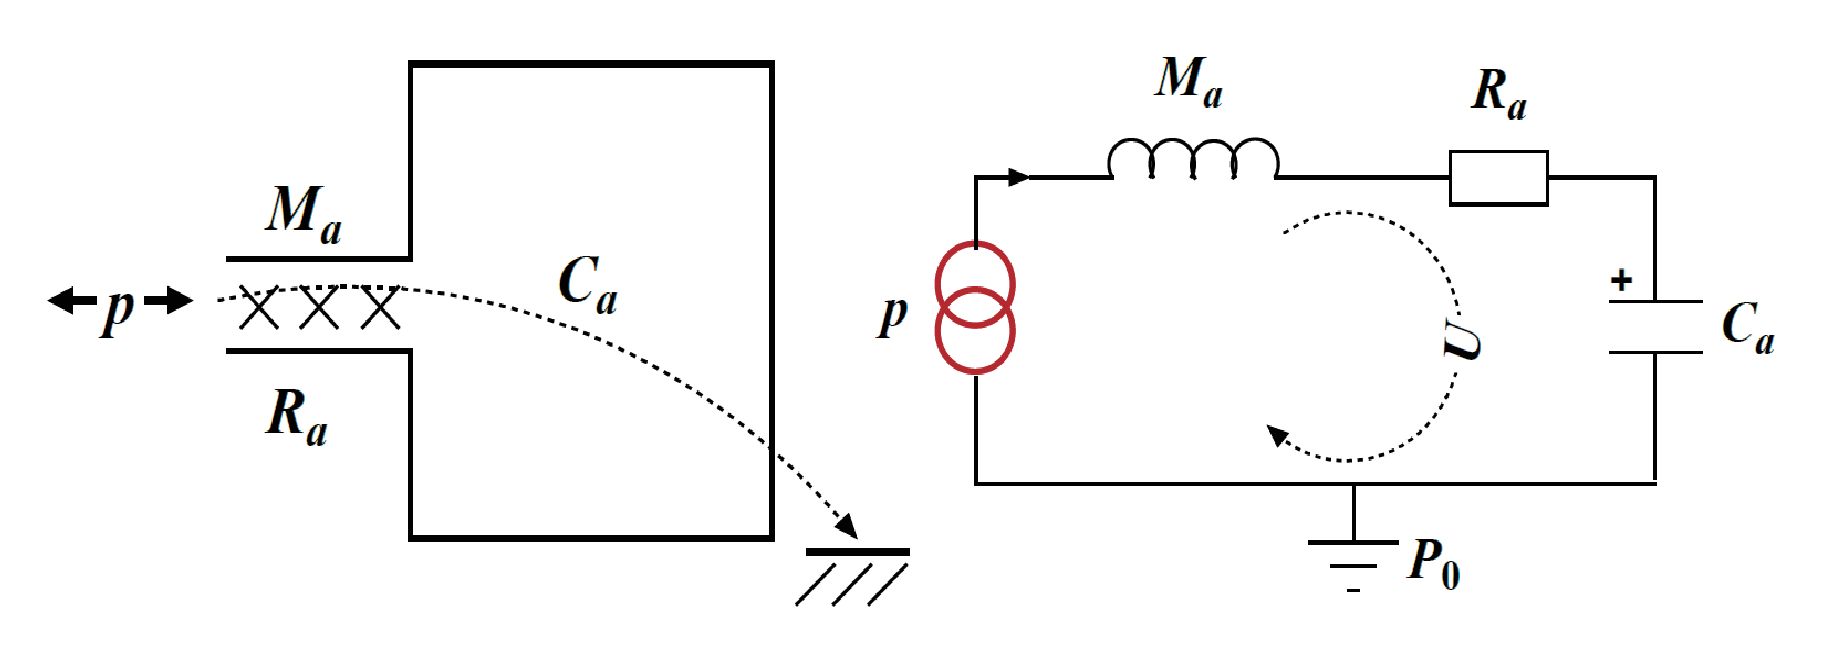
\includegraphics[width=1\textwidth]{images/fig2-3.eps} 
  \caption{亥姆霍兹共鸣器及其等效电路。}
  \label{fig_2_3}
\end{figure}

在定义了声顺,声阻,声质量之后,我们在这里探讨它们的连接和等效电路方法。如图 \ref{fig_2_3},亥姆霍兹共鸣器是一种由短管和刚性壁腔体构成的声学结构。该结构具体由截面积为$S$(半径为$a$)、长度为$l_0$的短管,与容积为$V_0$的刚性壁腔体联通而成,短管和腔体内部均充满密度为$\rho_0$的流体。对于所涉声波,设其波长为$\lambda$,且满足$\lambda \gg a, l_0, \sqrt[3]{V_0}$ 以及 $V_0 \gg Sl_0$ 的假设条件。在这种设定下,短管内的流体如同活塞般作整体运动,其质量$M_m = \rho_0Sl_0$ ,考虑到短管两端的声辐射效应,等效管长变为$l = l_0 + \Delta l =  l_0 + 1.7a$ 。此外,由于短管内空气高速运动,会受到管壁摩擦力,产生力阻$R_m$。在该声学结构中,管口会受到外界激励声压$p = P - P_0$的作用。我们以该结构的受力情况为研究对象,考虑到空气柱可能存在的力阻,在同时引入声质量$M_a$、声阻$R_a$和声顺$C_a$后,其关于声压$p$和体积速度$U$的振动方程可以写为
\begin{equation}\label{eq2-25}
  M_a\frac{dU}{dt} + R_aU + \frac{1}{C_a}\int Udt = p,
\end{equation}

不难发现,声学系统的控制方程(\ref{eq2-25})与电路系统的RLC电路的控制方程十分相似,并且在阻抗型类比中,电学元件和声学元件可以一一对应。RLC电路的控制方程为:
\begin{equation}\label{eq2-26}
  L_e\frac{dI}{dt} + R_eI + \frac{1}{C_e}\int Idt = E,
\end{equation}
对比方程(\ref{eq2-25})和方程(\ref{eq2-26}),在阻抗型声电类比关系里,声压$p$对应电压$E$,体速度$U$对应电流$I$,声质量$M_a$对应电感$L_e$,声顺$C_a$对应电容$C_e$,声阻$R_a$对应电阻$R_e$。元件两端的压强差$p = P - P_0$,对应于大气压强$P_0$的端点相当于“接地”,如图 \ref{fig_2_3}所示。这种方法可以扩展到更复杂的声学结构,前提条件是腔管结构尺寸和波长满足一定关系。这一理论帮助我们在第三章和第四章对声学哈密顿量进行理论建模。

 \section{腔体简正模式和格林函数}
 在上一小节我们介绍了声-电类比方法和等效电路模型。一方面,声波在腔管中作为一个分布变化的波函数,我可以用一些集总参数的电路元件来模拟其中的行为,需要有很多的限制条件。例如,我们必须在一个波长远大于尺寸的条件下对系统建模,这时腔体内声压随空间分布的函数近似为一个不变的常数,此后我们才可以用常数声压定义声容。而另一方面,在声学设计的时候,我们往往采用一些规则结构,例如长方体、圆柱体等。这使得其简正模式和频率可以非常容易地确定。因此,在本节中,我们将介绍腔体的简正模式和格林函数的关系,并以此研究腔体的耦合。

\subsection{刚性腔的简正模式}

\begin{figure}[h!]
  \centering
  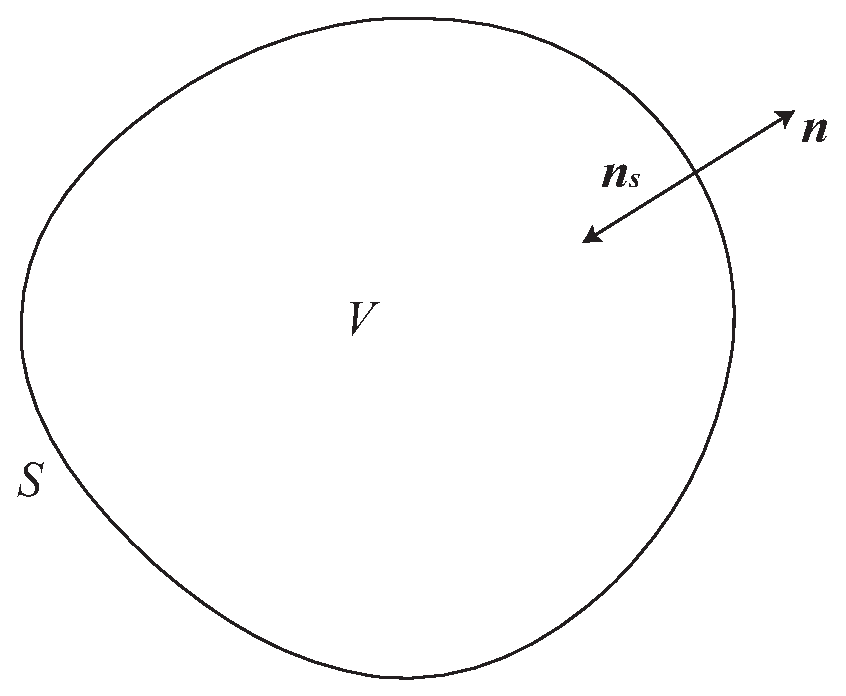
\includegraphics[width=0.5\textwidth]{images/fig2-4.eps} 
  \caption{腔体及其法向边界$\boldmath{n}$、内壁法向$\boldmath{n_s}$。}
  \label{fig_2_4}
\end{figure}

简正模式理论是求解有限空间声场的基本方法。其物理意义明确,每个简正模式对应一个驻波模式,简正频率即腔体共振频率,可在实验中测量。对于一些规则的结构,如长方体,圆柱体和球体,其简正模式和对应的共振频率可解析地求得,在此不再赘述。声源于腔内激发多种简正模式,腔内总声场为各激发模式的叠加。 在这里,我们探讨刚性壁面腔体的简正模式和展开。如图 \ref{fig_2_4}所示,设封闭区域$V$的边界为刚性边界$S$,边界的法向为$\symbfit{n}$(与内壁的法向$\symbfit{n_s}$相反)。在频率域中,声波方程和边界条件需满足:
\begin{equation}\label{eq2-27}
  \begin{split}
  \nabla^{2}p(\mathbf{r},\omega)+k_{0}^{2}p(\mathbf{r},\omega)&=-\mathfrak{I}(\mathbf{r},\omega)\quad(k_{0}=\omega/c_{0}),\\
  \mathbf{n}\cdot\nabla p(\mathbf{r},\omega)&\equiv\left.\frac{\partial p(\mathbf{r},\omega)}{\partial n}\right|_{S}=0,
  \end{split}
\end{equation}

其中,$\mathfrak{I}(\mathbf{r},\omega)$是体源分布。为了求声场分布,我们首先求$V$内的简正模式$\psi_{\lambda}(\mathbf{r},\omega_{\lambda})$和简正频率$\omega_{\lambda}$,它们是下列齐次问题的非零解:

\begin{equation}\label{eq2-28}
  \begin{split}
  \nabla^{2}\psi_{\lambda}(\mathbf{r},\omega_{\lambda})+k_{\lambda}^{2}\psi_{\lambda}(\mathbf{r},\omega_{\lambda})&=0\quad(k_{\lambda}=\omega_{\lambda}/c_{0}),\\
  \left.\frac{\partial\psi_{\lambda}(\mathbf{r},\omega_{\lambda})}{\partial n}\right|_{S}&=0,
  \end{split}
  \end{equation}

三维拉普拉斯算子$\nabla^{2}$在刚性边界条件下是厄米特对称算子,即简正模式$\psi_{\lambda}(\mathbf{r},\omega_{\lambda})$和简正频率$\omega_{\lambda}$同样具有三个基本性质:1. 简正频率$\omega_{\lambda}$是实数;2.简正模式$\psi_{\lambda}(\mathbf{r},\omega_{\lambda})$相互正交;3.简正系
\begin{equation}\label{eq2-29}
  \{\psi_{\lambda}(\mathbf{r},\omega_{\lambda}),\lambda = 0,1,2,\cdots\}
\end{equation}
构成完备系,即定义在$V$上的平方可积函数$p(\mathbf{r},\omega)$可作广义傅里叶级数展开:
\begin{equation}\label{eq2-30}
  p(\mathbf{r},\omega)\cong\sum_{\lambda = 0}^{\infty}a_{\lambda}\psi_{\lambda}(\mathbf{r},\omega_{\lambda}),
\end{equation}
其中,展开系数为
\begin{equation}\label{eq2-31}
  a_{\lambda}=\int_{V}p(\mathbf{r},\omega)\psi_{\lambda}^{*}(\mathbf{r},\omega_{\lambda})\mathrm{d}^{3}\mathbf{r},
\end{equation}
至此,我们可以通过求解方程(\ref{eq2-28}),得到声场函数的一组完备基函数。声压分布可以依据式(\ref{eq2-30})和(\ref{eq2-31}),由这组基表示。

\subsection{频域格林函数}
对于声场激发问题,将方程(\ref{eq2-30})代入(\ref{eq2-27})可得:
\begin{equation}\label{eq2-32}
  \sum_{\lambda = 0}^{\infty}a_{\lambda}[\nabla^{2}\psi_{\lambda}(\mathbf{r},\omega_{\lambda}) + k_{0}^{2}\psi_{\lambda}(\mathbf{r},\omega_{\lambda})]=-\mathfrak{I}(\mathbf{r},\omega),
\end{equation}
由方程(\ref{eq2-28})可得:
\begin{equation}\label{eq2-33}
  \sum_{\lambda = 0}^{\infty}a_{\lambda}(k_{0}^{2}-k_{\lambda}^{2})\psi_{\lambda}(\mathbf{r},\omega_{\lambda})=-\mathfrak{I}(\mathbf{r},\omega),
\end{equation}
利用$\psi_{\lambda}(\mathbf{r},\omega_{\lambda})$的正交归一性,有:
\begin{equation}\label{eq2-34}
  a_{\lambda}=\frac{1}{k_{\lambda}^{2}-k_{0}^{2}}\int_{V}\mathfrak{I}(\mathbf{r},\omega)\psi_{\lambda}^{*}(\mathbf{r},\omega_{\lambda})\mathrm{d}^{3}\mathbf{r},
\end{equation}
将上式代入方程(\ref{eq2-30})
\begin{equation}
\begin{split}
  p(\mathbf{r},\omega)&=\int_{V}\mathfrak{I}(\mathbf{r}',\omega)\left[\sum_{\lambda = 0}^{\infty}\frac{1}{k_{\lambda}^{2}-k_{0}^{2}}\psi_{\lambda}^{*}(\mathbf{r}',\omega_{\lambda})\psi_{\lambda}(\mathbf{r},\omega_{\lambda})\right]\mathrm{d}^{3}\mathbf{r}'\\
  &\equiv\int_{V}G_{0}(\mathbf{r},\mathbf{r}',\omega)\mathfrak{I}(\mathbf{r}',\omega)\mathrm{d}^{3}\mathbf{r}',
\end{split}
\end{equation}
其中,$G_0(\mathbf{r}, \mathbf{r}', \omega)$定义为:
\begin{equation}
  G_0(\mathbf{r}, \mathbf{r}', \omega) \equiv \sum_{\lambda = 0}^{\infty} \frac{1}{k_{\lambda}^{2} - k_{0}^{2}} \psi_{\lambda}^{*}(\mathbf{r}', \omega_{\lambda}) \psi_{\lambda}(\mathbf{r}, \omega_{\lambda}),
\end{equation}
显然,当$\mathfrak{I}(\mathbf{r}, \omega) = \delta(\mathbf{r}, \mathbf{r}')$时,方程:
\begin{equation}\label{eq2-27}
  \begin{split}
  \nabla^{2}G_{0}(\mathbf{r},\mathbf{r}',\omega)+k_{0}^{2}G_{0}(\mathbf{r},\mathbf{r}',\omega)&=-\delta(\mathbf{r},\mathbf{r}'),\\
  \left.\frac{\partial G_{0}(\mathbf{r},\mathbf{r}',\omega)}{\partial n}\right|_{S}&=0,
  \end{split}
\end{equation}
的解就是$G_0(\mathbf{r}, \mathbf{r}', \omega)$。因此,方程(\ref{eq2-27})就是格林函数$G_0(\mathbf{r}, \mathbf{r}', \omega)$用简正模式展开的表达式。在腔与腔之间为弱耦合时,我们认为求得的单个腔体的格林函数可以用刚性边界近似。随后,在没有体积源,腔的振动完全由边界提供。这时,我们就可以通过腔体耦合的边界情况及其格林函数积分公式求得声场分布:
\begin{equation}\label{eq2-38}
    p(\vec{r}) = -i\rho_0\omega \int_{\partial V} G(\vec{r},\vec{r}')v(\vec{r}')dS',
\end{equation}
这一理论帮助我们在第五章中实现了声学拓扑绝缘体的负耦合作用。

\section{小结}
在本章中,我们着重介绍了利用传统声学理论对声学拓扑绝缘体建模的理论工具,包括声电类比方法和简正模式与格林函数的推导。一方面,当结构尺寸远大于波长的时候,腔体内均匀振动通过声电类比天然近似为集总参数模型,这与离散的晶格结构存在着某种对应方式;另一方面当多个腔体处于同一共振模式的时候,我们认为它们的连接是弱耦合的,可以通过单个腔体格林函数进行声学近似,这使得整个问题得到简化。这两种方法有着不同的适用条件,在之后的章节中可以看到这两种方法在研究由腔管结构组成的拓扑绝缘体时非常有用。
